\documentclass[10pt,letterpaper]{amspset}
\usepackage{fullpage}
\usepackage{textcomp}
\usepackage{gensymb}
\usepackage{graphicx}
\usepackage{tikz}
\usetikzlibrary{angles, quotes}
\usepackage{amsmath}
\usepackage{pgfplots}
\usepackage{amsthm}
\usepackage{amssymb}
\usepackage{pst-coil}
\usepackage[utf8]{inputenc}
\usepackage[english]{babel}
\usepackage{empheq}

\usetikzlibrary{decorations.pathmorphing,patterns}
\pgfplotsset{compat=1.17}
\graphicspath{ {./images/} }
\notag
\newtheorem{theorem}{Theorem}
\newcommand*\widefbox[1]{\fbox{\hspace{2em}#1\hspace{2em}}}

% info for header block in upper right hand corner
\name{Brady Lamson}
\class{MATH 1120 SPRING 2021}
\assignment{Law of Sines and Cosines}
\duedate{Mar 21st}
\begin{document}

\problemlist{Law of Sines and Cosines: 

Section 11.2 Problems: 11--16, 22--27, 35--37

Section 11.3 Problems: 4--10, 11--16, 19--26}

\section{Introduction:}

\begin{problem}[Theorem 1. The Law of Sines:]
    Given a triangle with angle-side opposite pairs $(\alpha, a), (\beta, b), (\gamma, c)$, the following ratios hold:
    
    \[ \frac{sin(\alpha)}{a} = \frac{sin(\beta)}{b} = \frac{sin(\gamma)}{c}\]
    
    or, equivalently, 
    
    \[ \frac{a}{sin(\alpha)} = \frac{b}{sin(\beta)} = \frac{c}{sin(\gamma)}\]
\end{problem}

\begin{problem}[Theorem 2.]
    Suppose $(\alpha, a)$ and $(\gamma, c)$ are intended to be angle-side pairs in a triangle where $\alpha, a$ and $c$ are given. Let $h = c \cdot \sin(\alpha)$
    
    \begin{itemize}
        \item If $a < h$, then no triangle exists which satisfies the given criteria 
        \item If $a = h$, then $\gamma = \frac{\pi}{2}$ so exactly one (right) triangle exists which satisfies the criteria.
        \item If $h < a < c$, then two distinct triangles exist which satisfy the given criteria.
        \item if $a \geq c$, then $\gamma$ is acute and exactly one triangle exists which satisfies the given criteria.
    \end{itemize}
\end{problem}

\begin{problem}[Theorem 3. Law of Cosines:]
    Given a triangle with angle-side opposite pairs $(\alpha, a), (\beta, b), (\gamma, c)$, the following equations hold:
    
    \begin{align}
        \notag a^2 = b^2 + c^2 - 2 \cdot b \cdot c \cdot cos(\alpha) && b^2 = a^2 + c^2 - 2 \cdot a \cdot c \cdot cos(\beta) && c^2 = a^2 + b^2 - 2 \cdot a \cdot b \cdot cos(\gamma)
    \end{align}
    
    or, solving for the cosine in each equation, we have
    
    \begin{align}
        \notag \cos(\alpha) = \frac{b^2 + c^2 - a^2}{2bc} && \cos(\beta) = \frac{a^2 + c^2 - b^2}{2ac} && \cos(\gamma) = \frac{a^2 + b^2 - c^2}{2ab}
    \end{align}
\end{problem}

\begin{problem}[Converting Between Radians and Degrees:]
    Here for convenience.
    
    Converting from degrees to radians,
    
    \[1\degree \cdot \frac{1\pi}{180\degree} = \text{Radians}\]
    
    Converting from radians to degrees,
    
    \[1 \; \text{radian} \cdot \frac{180\degree}{\pi} = \text{Degrees}\]
\end{problem}
    
\pagebreak

\section{11.2: Law of Sines: Problems 11--16, 22--27, 35--37}

\begin{problem}
    In Exercises 11--16, solve for the remaining side(s) and angle(s) if possible. As in the text, $(\alpha, a), (\beta, b), (\gamma, c)$ are angle-side opposite pairs.
\end{problem}

\begin{problem}[11.]
    $\alpha = 42\degree$, $a = 39$, $b = 23.5$
\end{problem}

\begin{solution}
    \[\alpha = 42\degree \cdot \frac{\pi}{180\degree} = 0.733 \; \text{radians}\]
    
    To start, since we know $\alpha$, $a$ and $b$ we can use the law of sines to solve for $\beta$. 
    
    \begin{align}
        \frac{sin(\alpha)}{a} &= \frac{sin(\beta)}{b} \\
        \sin(\beta) &= \frac{b \cdot \sin(\alpha)}{a} \\
        \sin(\beta) &= \frac{23.5 \cdot \sin(0.733)}{39} \\
        \sin(\beta) &= 0.403 \\
        \beta &= arcsin(0.403)
    \end{align}
    \[\boxed{ \beta \approx 0.4149 \; \text{radians}  }\]
    
    Now we solve for $\gamma$. We know that $\alpha + \beta + \gamma = \pi$ for all triangles. 
    
    \begin{align}
        \alpha + \beta + \gamma &= \pi \\
        0.733 + 0.4149 + \gamma &= \pi \\
        \gamma &= \pi - 0.733 - 0.4149
    \end{align}
    \[\boxed{  \gamma \approx 1.994 \; \text{radians}  }\]
    
    All we do now is the same as the first step when we solved for $\beta$, this time solving for $c$ instead. 
    
    \begin{align}
        \frac{\sin(\alpha)}{a} &= \frac{\sin(\gamma)}{c} \\
        c &= \frac{\sin(\gamma) \cdot a}{\sin(\alpha)} \\
        c &= \frac{\sin(1.994) \cdot 39}{\sin(0.733)}
    \end{align}
    \[\boxed{ c \approx 53.145  }\]
\end{solution}

\begin{problem}[12.]
    $\gamma = 53\degree$, $\alpha = 53\degree$, $c = 28.01$
\end{problem}

\begin{solution}
    \[\alpha \; \text{and} \; \gamma = 53\degree \cdot \frac{1\pi}{180\degree} = 0.925 \; \text{radians}\]
    
    Since $\alpha$ and $\gamma$ are the same we can say that $a = c$
    \[\boxed{a = 28.01}\]
    
    Calculating $\beta$:
    \begin{align}
        \alpha + \beta + \gamma = \pi \\
        \beta = \pi - 2(0.925)
    \end{align}
    \[\boxed{ \beta \approx 1.29 \; \text{radians}  }\]
    
    Calculating $b$:
    \begin{align}
        \frac{\sin(\alpha)}{a} &= \frac{\sin(\beta)}{b} \\
        b &= \frac{\sin(\beta) \cdot a}{\sin(\alpha)} \\
        b &= \frac{\sin(1.29) \cdot 28.01}{\sin(0.925)}
    \end{align}
    \[\boxed{ b \approx 33.699  }\]
\end{solution}

\begin{problem}[13.]
    $a = 57$, $\alpha = 6\degree$, $b = 100$
\end{problem}

\begin{solution}
   \[\alpha = 6\degree \cdot \frac{\pi}{180\degree} = 0.1047 \; \text{radians}\] 
   
   Calculating $\beta$:
   \begin{align}
       \frac{sin(\alpha)}{a} &= \frac{sin(\beta)}{b} \\
       \sin(\beta) &= \frac{b \cdot \sin(\alpha)}{a} \\
       \sin(\beta) &= \frac{100 \cdot \sin(0.1047)}{57} \\
       \sin(\beta) &= 0.1833 \\
       \beta &= arcsin(0.1833)
   \end{align}
   \[\boxed{ \beta \approx 0.1843 \; \text{radians}  }\]
    
   Calculating $\gamma$:
    \begin{align}
        \alpha + \beta + \gamma &= \pi \\
        0.1047 + 0.1843 + \gamma &= \pi \\
        \gamma &= \pi - 0.1047 - 0.1843
    \end{align}
    \[\boxed{  \gamma \approx 2.853 \; \text{radians}  }\]
    
    Calculating $c$:
    \begin{align}
        \frac{\sin(\alpha)}{a} &= \frac{\sin(\gamma)}{c} \\
        c &= \frac{\sin(\gamma) \cdot a}{\sin(\alpha)} \\
        c &= \frac{\sin(2.853) \cdot 57}{\sin(0.1047)}
    \end{align}
    \[\boxed{ c \approx 155.225  }\]
    
    Testing for number of solutions: 
    \begin{align}
        h &= c \cdot \sin(\alpha) \\
        h &= 155.225 \cdot \sin(0.1047) \\
        h &\approx 16.222 \\
    \end{align}
    
    What we find here is that $h < a < c$, so we have \textbf{two} possible solutions to this problem. We aren't done yet. Let's think again about exactly \emph{what} we're trying to even do here. We're given a single angle and two sides at the beginning. Those are our restrictions. The problem is asking what triangles, if any at all, can be made using these restrictions. In other words, we can play around with what isn't restricted. That being 1 side and 2 angles. 
    
    \pagebreak
    
    Looking again at what we're given at the beginning, let's solve for $\beta$. To really hammer home why this can be done using two different values of $\beta$ let's use a basic example.
    
    \[sin(\theta) = \frac{1}{2}\]
    \[arcsin\left( \frac{1}{2} \right) = \theta\]
    \[\theta = \frac{\pi}{6}, \frac{5\pi}{6}, \frac{13\pi}{6}, \frac{17\pi}{6}, ...\]
    \[\theta = 30\degree, 150\degree, 390\degree, 510\degree, ...\]
    
    There are multiple possible options here depending on what you're restricted to! \emph{So}, to get to the point solving for our other value of $\beta$ is easy! We subtract it from $\pi$ (or $180\degree$)! Since $\alpha$ is set to $6\degree$ we're restricted to $0 < \beta < 174\degree$. If the result doesn't fall within that range of we know it can't be done. Note: $174\degree \approx 3.036$ radians.
    
    Solving for $\beta_1$:
    \begin{align}
        \beta_0 + \beta_1 = \pi \\
        \beta_1 = \pi - \beta_0 \\
        \beta_1 = \pi - 0.1843
    \end{align}
    \[\boxed{\beta_1 \approx 2.957 \; \text{radians}}\]
    
    Solving for $\gamma_1$: 
    \begin{align}
        \beta_1 + \gamma_1 \approx 3.036 \\
        \gamma_1 \approx 3.036 - 2.957
    \end{align}
    \[\boxed{\gamma_1 \approx 0.079 \; \text{radians}}\]
    
    Both fall within our restricted range so we're good to go! All we do now is solve for $c$ and we're done! 
    
    Calculating $c_1$:
    \begin{align}
        \frac{\sin(\beta_1)}{b} &= \frac{\sin(\gamma_1)}{c_1} \\
        c_1 &= \frac{\sin(\gamma_1) \cdot b}{\sin(\beta_1)} \\
        c_1 &= \frac{\sin(0.079) \cdot 100}{\sin(2.957)}
    \end{align}
    \[\boxed{ c_1 \approx 42.99  }\]
    
    \begin{subequations}
        \begin{empheq}[box=\widefbox]{align}
            a = 57 && b = 100 && c \approx 155.225 \\
            \alpha \approx 0.1047 \; \text{rad} && \beta \approx 0.1843 \; \text{rad} && \gamma \approx 2.853 \; \text{rad} \\
            \\
            a = 57 && b = 100 && c_1 \approx 42.99 \\
            \alpha \approx 0.1047 \; \text{rad} && \beta_1 \approx 2.957 \; \text{rad} && \gamma_1 \approx 0.079 \; \text{rad}
        \end{empheq}
    \end{subequations}
\end{solution}

\begin{problem}[14]
    $\gamma = 74.6\degree$, $c = 3$, $a = 3.05$
\end{problem}

\begin{solution}
    \[\gamma = 74.6\degree \cdot \frac{\pi}{180\degree} = 1.302 \; \text{radians}\] 
    
    Calculating $h$: ($\gamma, c$ and $a$ are given)
    \begin{align}
        h &= a \cdot \sin(\gamma) \\
        h &= 3.05 \cdot \sin(1.302) \\
        h &\approx 2.94 \\
        2.94 &< 3 < 3.05 \\
        h &< c < a
    \end{align}
    
    Going into this we know we will have two possible solutions to work with. Let's get started. \medskip
    
    Calculating $\alpha$:
    \begin{align}
       \frac{sin(\alpha)}{a} &= \frac{sin(\gamma)}{c} \\
       \sin(\alpha) &= \frac{\sin(\gamma) \cdot a}{c} \\
       \sin(\alpha) &= \frac{\sin(1.302) \cdot 3.05}{3} \\
       \sin(\alpha) &= 0.9802 \\
       \alpha &= \arcsin(0.9802)
   \end{align}
   \[\boxed{ \alpha \approx 1.3712 \; \text{radians}  }\]
   
   Calculating $\beta$:
   \begin{align}
       \beta = \pi - \alpha - \gamma \\
       \beta = \pi - 1.3712 - 1.302
   \end{align}
   \[\boxed{\beta \approx 0.4683 \; \text{radians}}\]
   
   Calculating $b$:
    \begin{align}
       \frac{sin(\gamma)}{c} &= \frac{sin(\beta)}{b} \\
       b &= \frac{\sin(\beta) \cdot c}{\sin(\gamma)} \\
       b &= \frac{\sin(0.4683) \cdot 3}{\sin(1.302)}
   \end{align}
   \[\boxed{ b \approx 1.405 }\]
   
   First triangles done, let's get our alternate value of $\alpha$. \pagebreak
   
   Calculating $\alpha_1$:
   \begin{align}
        \alpha_0 + \alpha_1 = \pi \\
        \alpha_1 = \pi - \alpha_0 \\
        \alpha_1 = \pi - 1.3712
   \end{align}
   \[\boxed{\alpha_1 \approx 1.7704 \; \text{radians}}\]
   
   To calculate $\beta_1$ we need to know our restricted range. We can define that as $0 < \beta_1 < x$ if we let $x = \pi - \gamma$. \bigskip
   
   Calculating $\beta_1$ (Range is $0 < \beta_1 < 104\degree$).
   \hspace{1mm} Note: $105.4\degree \approx 1.815$ radians.
    \begin{align}
        \alpha_1 + \beta_1 = 1.8396 \\
        \beta_1 = 1.8396 - 1.7704
    \end{align}
    \[\boxed{\beta_1 \approx 0.0692 \; \text{radians}}\]
    
    Calculating $b_1$
    \begin{align}
       \frac{sin(\gamma)}{c} &= \frac{sin(\beta_1)}{b_1} \\
       b_1 &= \frac{\sin(\beta_1) \cdot c}{\sin(\gamma)} \\
       b_1 &= \frac{\sin(0.0692) \cdot 3}{\sin(1.302)}
   \end{align}
   \[\boxed{ b_1 \approx 0.215 }\]
   
    \begin{subequations}
        \begin{empheq}[box=\widefbox]{align}
            a = 3.05 && b \approx 1.405 && c = 3 \\
            \alpha \approx 1.3712 \; \text{rad} && \beta \approx 0.4683 \; \text{rad} && \gamma = 1.302 \; \text{rad} \\
            \\
            a = 3.05 && b_1 \approx 0.215 && c = 3 \\
            \alpha_1 \approx 1.7704 \; \text{rad} && \beta_1 \approx 0.0692 \; \text{rad} && \gamma = 1.302 \; \text{rad}
        \end{empheq}
    \end{subequations}
\end{solution}

\begin{problem}[15.]
    $\beta = 102\degree, b = 16.75, c = 13$
\end{problem}

\begin{solution}
    Calculating $h$: ($\beta, b$ and $c$ are given)
    \begin{align}
        h &= c \cdot \sin(\beta) \\
        h &= 13 \cdot \sin(102\degree) \\
        h &\approx 12.7159 \\
        12.7159 &< 13 < 16.75 \\
    \end{align}
    
    Because $b \geq c$, $\gamma$ is acute and we need to solve for one triangle. \medskip
    
    Calculating $\gamma$:
    \begin{align}
       \frac{sin(\beta)}{b} &= \frac{sin(\gamma)}{c} \\
       \sin(\gamma) &= \frac{\sin(\beta) \cdot c}{b} \\
       \sin(\gamma) &= \frac{\sin(102\degree) \cdot 13}{16.75} \\
       \sin(\gamma) &= 0.7592 \\
       \gamma &= \arcsin(0.7592)
   \end{align}
   \[\boxed{ \gamma \approx 49.39\degree}\]
   
   Calculating $\alpha$:
   \begin{align}
       \alpha = 180\degree - \beta - \gamma \\
       \alpha = 180\degree - 102\degree - 43.39\degree 
   \end{align}
   \[\boxed{\alpha \approx 28.61 \degree}\]
   
   Calculating $a$:
    \begin{align}
       \frac{sin(\alpha)}{a} &= \frac{sin(\beta)}{b} \\
       a &= \frac{\sin(\alpha) \cdot b}{\sin(\beta)} \\
       a &= \frac{\sin(28.61\degree) \cdot 16.75}{\sin(102\degree)}
   \end{align}
   \[\boxed{ a \approx 8.199 }\]
   
    \begin{subequations}
        \begin{empheq}[box=\widefbox]{align}
            a \approx 8.20 && b = 16.75 && c = 13 \\
            \alpha \approx 28.61\degree && \beta = 102\degree && \gamma \approx 49.39\degree
        \end{empheq}
    \end{subequations}
\end{solution}

\begin{problem}[16.]
    $\beta = 102\degree, b = 16.75, c = 18$
\end{problem}

\begin{solution}
    Calculating $h$: ($\beta, b$ and $c$ are given)
    \begin{align}
        h &= c \cdot \sin(\beta) \\
        h &= 18 \cdot \sin(102\degree) \\
        h &\approx 17.6 \\
        16.75 &< 17.6 < 18 \\
        b &< h < c
    \end{align}
    
    Because $b$ is less than $h$ there are no triangles that satisfy our restrictions. 
\end{solution}


\begin{problem}[22]
    Using a right triangle with a horizontal leg of length 100 and vertical leg with length 7, show that a $7\%$ grade means that the road (hypotenuse) makes about a $4\degree$ angle with the horizontal. (It will not be exactly $4\degree$ , but it’s pretty close.)
\end{problem}

\begin{solution}
    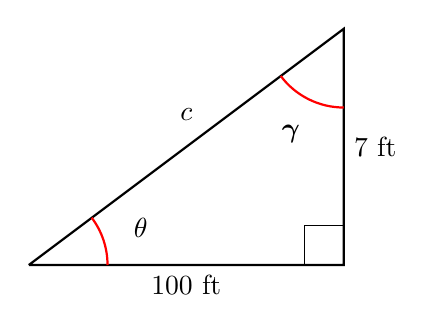
\begin{tikzpicture}
        % Draw triangle
        \draw[black, thick] 
            (0,0)
                coordinate (a)
            -- (4,0) 
                coordinate (b)
                node[midway, below] {$100$ ft}
            -- (4,3) 
                coordinate (c)
                node [midway, right] {$7$ ft}
            -- (0,0) 
                node[midway, above=2mm] {$c$};
        % Draw interior angles
            \pic [draw=red, thick, "$\boldsymbol{\gamma}$", angle eccentricity=1.5, angle radius=1cm] 
                {angle = a--c--b};
            \pic [draw=red, thick, "$\theta$", angle eccentricity=1.5, angle radius = 1cm]
                {angle = b--a--c};
        % Add the right angle signifiers 
            \draw[] (4,0) rectangle (3.5,0.5);
    \end{tikzpicture}
    
    All we really need to do here is take the tangent of $\theta$, do some arctangent nonsense and then convert our value of $\theta$ into degrees! Easy.
    
    \begin{align}
        \tan(\theta) &= \frac{7}{100} \\
        \theta &= \arctan \left( \frac{7}{100} \right) \\
        \theta &\approx 0.0699 \; \text{radians} \\
        \theta &\approx 0.0699 \; \text{radians} \cdot \frac{180\degree}{\pi} 
    \end{align}
    \[\boxed{\theta \approx 4\degree}\]
\end{solution}


\begin{problem}[23]
    What grade is given by a $9.65\degree$ angle made by the road and the horizontal?
\end{problem}

\begin{solution}
    \begin{align}
        \phi &= 9.65\degree \\
        \phi &\approx 9.65\degree \cdot \frac{\pi}{180\degree} \\
        \phi &\approx 0.168 \; \text{radians} \\
        \tan(0.168) &\approx 0.17
    \end{align}
    \[\boxed{\approx 17\%}\]
\end{solution}

\begin{problem}[24]
    Along a long, straight stretch of mountain road with a $7\%$ grade, you see a tall tree standing perfectly plumb alongside the road. From a point 500 feet downhill from the tree, the angle of inclination from the road to the top of the tree is $6\degree$. Use the Law of Sines to find the height of the tree.
\end{problem}

\begin{solution}
    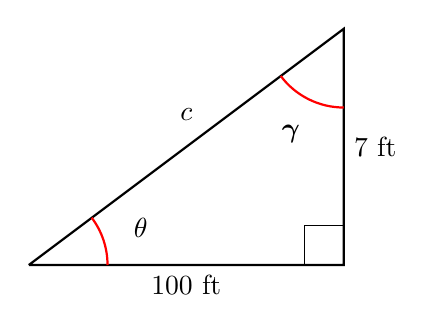
\begin{tikzpicture}
        % Draw triangle
        \draw[black, thick] 
            (0,0)
                coordinate (a)
            -- (4,0) 
                coordinate (b)
                node[midway, below] {$100$ ft}
            -- (4,3) 
                coordinate (c)
                node [midway, right] {$7$ ft}
            -- (0,0) 
                node[midway, above=2mm] {$c$};
        % Draw interior angles
            \pic [draw=red, thick, "$\boldsymbol{\gamma}$", angle eccentricity=1.5, angle radius=1cm] 
                {angle = a--c--b};
            \pic [draw=red, thick, "$\theta$", angle eccentricity=1.5, angle radius = 1cm]
                {angle = b--a--c};
        % Add the right angle signifiers 
            \draw[] (4,0) rectangle (3.5,0.5);
    \end{tikzpicture}
    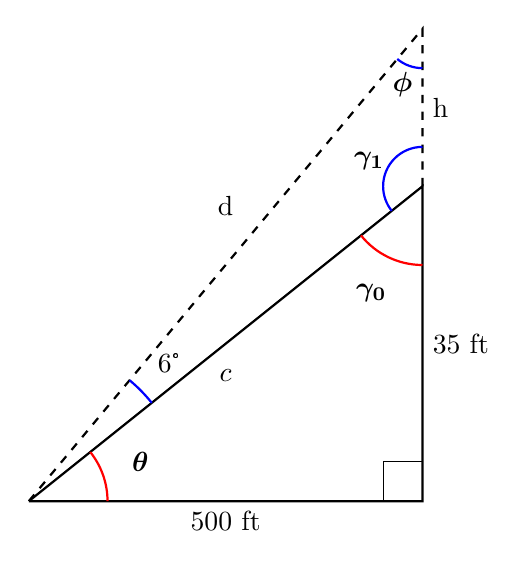
\begin{tikzpicture}
        % Draw triangle
        \draw[black, thick] 
            (0,0)
                coordinate (a)
            -- ++(5,0) 
                coordinate (b)
                node[midway, below] {$500$ ft}
            -- ++(0,4) 
                coordinate (c)
                node [midway, right] {$35$ ft}
            -- (a) 
                node[midway, below=2mm] {$c$};
        % Draw upper triangle
            \draw[dashed, thick]
                (c)
                -- ++(0,2) coordinate (d)
                    node [midway, right] {h}
                -- (a)
                    node [midway, above=0.5cm] {d};
        % Draw interior angles for primary triangle
            \pic [draw=red, thick, "$\boldsymbol{\gamma_0}$", angle eccentricity=1.5, angle radius=1cm] 
                {angle = a--c--b};
            \pic [draw=red, thick, "$\boldsymbol{\theta}$", angle eccentricity=1.5, angle radius = 1cm]
                {angle = b--a--c};
            % Add the right angle signifiers 
                \draw[] (5,0) rectangle (4.5,0.5);
        % Draw interior angles for secondary triangle
            \pic [draw=blue, thick, "$\boldsymbol{\gamma_1}$", angle eccentricity=1.5, angle radius=0.5cm] 
                {angle = d--c--a};
            \pic [draw=blue, thick, "$\boldsymbol{\phi}$", angle eccentricity=1.5, angle radius = 0.5cm]
                {angle = a--d--c};
            \pic [draw=blue, thick, "$6\degree$", angle eccentricity=1.25, angle radius = 2cm]
                {angle = c--a--d};            
    \end{tikzpicture}
    
    We now have two functional diagrams describing what's going on here. It's important to note that $\theta$ here is known. We calculated it in problem 22. We know its value is $4\degree$. This knowledge allows us to snowball out of control a bit here. Because we know $\theta$ AND that the angle attached to it is $6\degree$ what we can do is solve for $\phi$ by treating this as one large right triangle with angles $10\degree, 90\degree$, and $\phi$!
    
    \[\phi = 180\degree - 10\degree - 90\degree\]
    \[\phi = 80\degree\]
    
    From here we can solve for the angle next to $\gamma$. We'll refer to it as $\gamma_1$. Our dotted triangle has angles $6\degree, 80\degree$, and $\gamma_1$.
    \[\gamma_1 = 180\degree - 80\degree - 6\degree\]
    \[\gamma_1 = 94\degree\]
    
    For us to use the law of sines we need to know 2 angles and a side. We can solve for $c$ using the Pythagorean Theorem on the right triangle to get that one side we need. 
    
    \[c^2 = 500^2 + 35^2\]
    \[c = \sqrt{500^2 + 35^2}\]
    \[c = \sqrt{251225} \; \text{or} \; \approx 501\]
    
    Now the law of sines finally comes into play. 
    
    \begin{align}
        \frac{\sin(\phi)}{c} = \frac{sin(6\degree)}{h} \\
        h = \frac{\sin(6\degree) \cdot c}{\sin(\phi)} \\
        h \approx \frac{\sin(6\degree) \cdot 501}{\sin(80\degree)}
    \end{align}
    \[\boxed{h \approx 53ft}\]
\end{solution}

\begin{problem}[35]
    Discuss with yourself (because it's a pandemic and you're perpetually lonely) why knowing only the three angles of a triangle is not enough to determine any of the sides.
\end{problem}

\begin{solution}
    The thing about the law of sines is that it describes a relationship between the angles and sides of a triangle. Knowing just angles can result in an infinite number of answers that fit. Meanwhile, knowing one side gives you insight into the relationship between that side and its corresponding angle. That insight is what lets you solve for the rest of the sides. Without knowledge on at least one side you're left with an infinite number of possibilities. 
\end{solution}

\begin{problem}[36]
    Discuss with yourself (because it's a pandemic and you're perpetually lonely) why the Law of Sines cannot be used to find the angles in the triangle when only the three sides are given. Also discuss what happens if only two sides and the angle between them are given. (Said another way, explain why the Law of Sines cannot be used in the SSS and SAS cases.)
\end{problem}

\begin{solution}
    Much like I just said, the law of sines simply isn't built for that purpose. A law that describes the relationship between angles and sides cannot be used to \emph{find} the relationship between sides and unknown angles. Thankfully, that's why sine, cosine and tangent exist in the first place. You can always construct a right triangle out of the triangle you're given and go from there. If you know all three sides you're making more work for yourself by trying to use the laws anyway. 
    
    As for the second situation, things get kind of funny. Let's try and present this situation in an equation to see what it looks like.
    
    \[\frac{\sin(\alpha)}{a} = \frac{\sin(\beta)}{b} = \frac{\sin(\gamma)}{c} \]
    
    \[\frac{\sin(15\degree)}{a} = \frac{\sin(\beta)}{20} = \frac{\sin(\gamma)}{35} \]
    
    Going off of this, we don't actually \emph{know} anything about the relationship here. We don't have the insight we need to do anything with this law.
\end{solution}

\section{11.3: Law of Cosines: Problems: 4--10, 11--16, 19--26}
\begin{problem}
    In exercises 4--10, use the Law of Cosines to find the remaining side(s) and angle(s), if possible.
\end{problem}

\begin{problem}[4]
    $a=3$, $b=4$, $\gamma=90\degree$    
\end{problem}
    
\begin{solution}
    Not too much to explain here, I hope the math speaks for itself. I kind of just utilize the law of cosines and change it up depending on what I'm solving for. Refer to the introduction if you're lost. \bigskip
    
    Calculating $c$:
    \begin{align}
        c^2 &= a^2 + b^2 - (2 \cdot a \cdot b \cdot \cos(\gamma)) \\
        c^2 &= 3^2 + 4^2 - (2 \cdot 3 \cdot 4 \cdot \cos(90\degree)) \\
        c^2 &= 9 + 16 - (0) \hspace{+5mm} \text{note:} \; (\cos(90) = 0) \\
        c &= 5
    \end{align}
    
    Calculating $\alpha$
    \begin{align}
        \cos(\alpha) = \frac{b^2 + c^2 - a^2}{2 \cdot b \cdot c} && \alpha = \arccos \left( \frac{32}{40} \right) \\
        \alpha = \arccos \left( \frac{b^2 + c^2 - a^2}{2 \cdot b \cdot c} \right) && \alpha \approx 0.6435 \; \text{radians} \\ 
        \alpha = \arccos \left( \frac{4^2 + 5^2 - 3^2}{2 \cdot 4 \cdot 5} \right) && \boxed{\alpha \approx 36.87\degree}
    \end{align}
    
    Calculating $\beta$
    \begin{align}
        \cos(\beta) = \frac{a^2 + c^2 - b^2}{2 \cdot a \cdot c} && \beta = \arccos \left( \frac{18}{30} \right) \\
        \beta = \arccos \left( \frac{a^2 + c^2 - b^2}{2 \cdot a \cdot c} \right) && \beta \approx 0.9273 \; \text{radians} \\ 
        \beta = \arccos \left( \frac{3^2 + 5^2 - 4^2}{2 \cdot 3 \cdot 5} \right) && \boxed{\beta \approx 53.13\degree}
    \end{align}
    
    \begin{subequations}
        \begin{empheq}[box=\widefbox]{align}
            a = 3 && b = 4 && c = 5 \\
            \alpha \approx 36.87\degree && \beta \approx 53.13\degree && \gamma = 90\degree
        \end{empheq}
    \end{subequations}
\end{solution}

\begin{problem}[6]
    $a=7$, $b=10$, $c=13$    
\end{problem}
    
\begin{solution}
    Looking at our givens we have all three sides and no angles. That's fine. We'll just do this just like we solved for $\beta$ and $\alpha$ in the previous problem.
    
    Calculating $\alpha$:
    \begin{align}
        \cos(\alpha) = \frac{b^2 + c^2 - a^2}{2 \cdot b \cdot c} && \alpha = \arccos \left( \frac{220}{260} \right) \\
        \alpha = \arccos \left( \frac{b^2 + c^2 - a^2}{2 \cdot b \cdot c} \right) && \alpha \approx 0.562 \; \text{radians} \\ 
        \alpha = \arccos \left( \frac{10^2 + 13^2 - 7^2}{2 \cdot 10 \cdot 13} \right) && \boxed{\alpha \approx 32.2\degree}
    \end{align}
    
    Calculating $\beta$
    \begin{align}
        \cos(\beta) = \frac{a^2 + c^2 - b^2}{2 \cdot a \cdot c} && \beta = \arccos \left( \frac{118}{182} \right) \\
        \beta = \arccos \left( \frac{a^2 + c^2 - b^2}{2 \cdot a \cdot c} \right) && \beta \approx 0.4647 \; \text{radians} \\ 
        \beta = \arccos \left( \frac{7^2 + 13^2 - 10^2}{2 \cdot 7 \cdot 13} \right) && \boxed{\beta \approx 49.58 \degree}
    \end{align}
    
    Calculating $\gamma$: 
    \begin{align}
        \cos(\gamma) = \frac{a^2 + b^2 - c^2}{2 \cdot a \cdot b} && \gamma = \arccos \left( -\frac{20}{140} \right) \\
        \gamma = \arccos \left( \frac{a^2 + b^2 - c^2}{2 \cdot a \cdot b} \right) && \gamma \approx 1.714 \; \text{radians} \\ 
        \gamma = \arccos \left( \frac{7^2 + 10^2 - 13^2}{2 \cdot 7 \cdot 10} \right) && \boxed{\gamma \approx 98.21 \degree}
    \end{align}
    
    \begin{subequations}
        \begin{empheq}[box=\widefbox]{align}
            a = 7 && b = 10 && c = 13 \\
            \alpha \approx 32.2\degree && \beta \approx 49.58\degree && \gamma \approx 98.21 \degree
        \end{empheq}
    \end{subequations}
\end{solution}

\begin{problem}[8]
    $a=300$, $b=302$, $c=48$    
\end{problem}
    
\begin{solution}
    You know the drill.
    
    Calculating $\alpha$:
    \begin{align}
        \cos(\alpha) = \frac{b^2 + c^2 - a^2}{2 \cdot b \cdot c} && \alpha = \arccos \left( \frac{3508}{28992} \right) \\
        \alpha = \arccos \left( \frac{b^2 + c^2 - a^2}{2 \cdot b \cdot c} \right) && \alpha \approx 1.4495 \; \text{radians} \\ 
        \alpha = \arccos \left( \frac{302^2 + 48^2 - 300^2}{2 \cdot 302 \cdot 48} \right) && \boxed{\alpha \approx 83.05024 \degree}
    \end{align}
    
    Calculating $\beta$
    \begin{align}
        \cos(\beta) = \frac{a^2 + c^2 - b^2}{2 \cdot a \cdot c} && \beta = \arccos \left( \frac{2304}{28800} \right) \\
        \beta = \arccos \left( \frac{a^2 + c^2 - b^2}{2 \cdot a \cdot c} \right) && \beta \approx 1.5326 \; \text{radians} \\ 
        \beta = \arccos \left( \frac{300^2 + 48^2 - 302^2}{2 \cdot 300 \cdot 48} \right) && \boxed{\beta \approx 87.8 \degree}
    \end{align}
    
    Calculating $\gamma$: 
    \begin{align}
        \cos(\gamma) = \frac{a^2 + b^2 - c^2}{2 \cdot a \cdot b} && \gamma = \arccos \left( \frac{178900}{181200} \right) \\
        \gamma = \arccos \left( \frac{a^2 + b^2 - c^2}{2 \cdot a \cdot b} \right) && \gamma \approx 0.1595 \; \text{radians} \\ 
        \gamma = \arccos \left( \frac{300^2 + 302^2 - 48^2}{2 \cdot 300 \cdot 302} \right) && \boxed{\gamma \approx 9.14 \degree}
    \end{align}
    
    \begin{subequations}
        \begin{empheq}[box=\widefbox]{align}
            a = 300 && b = 302 && c = 48 \\
            \alpha \approx 83.05\degree && \beta \approx 87.8\degree && \gamma \approx 9.14 \degree
        \end{empheq}
    \end{subequations}
\end{solution}

\begin{problem}[19]
    A geologist wants to measure the diameter of a crater. From her camp, it is 4 miles to the northern-most point of the crater and 2 miles to the southern-most point. If the angle between the two lines of sight is $117\degree$ , what is the diameter of the crater? Round your answer to the nearest hundredth of a mile.
\end{problem}

\begin{solution}
    First let's make a diagram of what we're working with. \bigskip
    
    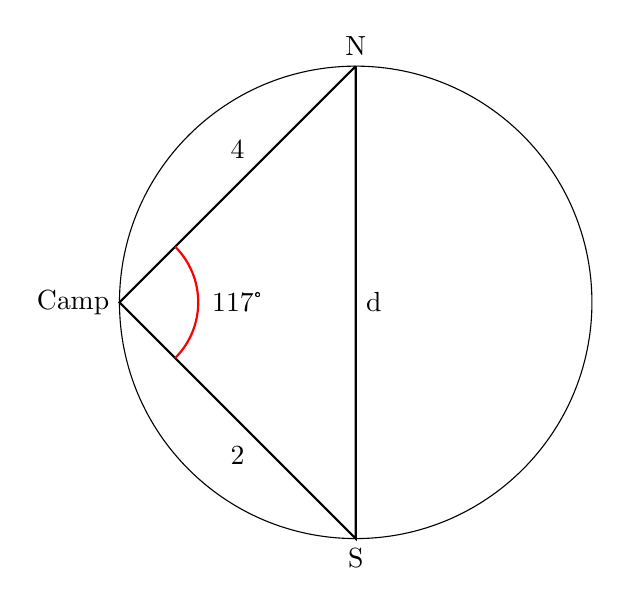
\begin{tikzpicture}
        \draw[] (0,0) circle (3);
        \draw[thick] 
        (0,3) coordinate (a) 
            node [above] {N}
            node [midway, sloped, right] {d}
        -- (0,-3) coordinate (b) [below] 
            node {S}
        -- (-3,0) coordinate (c)
            node [left] {Camp}
            node [midway, below=2mm] {2}
        -- (0,3)
            node[midway, above=2mm] {4};
        \pic [draw=red, thick, "$117 \degree$", angle eccentricity=1.5, angle radius = 1cm]
            {angle = b--c--a};
    \end{tikzpicture}
    
    We need to use the law of cosines to solve for $c$! We'll let $c = d$, $a = 4$, $b = 2$ and $\gamma = 117\degree$. \medskip
    
    Calculating $c$:
    \begin{align}
        c^2 &= a^2 + b^2 - (2 \cdot a \cdot b \cdot \cos(\gamma)) \\
        d^2 &= 4^2 + 2^2 - (2 \cdot 4 \cdot 2 \cdot \cos(117\degree)) \\
        d^2 &\approx 16 + 4 - (16 \cdot -0.454)\\
        d &= \sqrt{20 + 7.26}
    \end{align}
    
    \[\boxed{d \approx 5.22 \; \text{miles}}\]
\end{solution}

\begin{problem}[20]
    From the Pedimaxus International Airport a tour helicopter can fly to Cliffs of Insanity Point by following a bearing of N$8.2\degree$ E for 192 miles and it can fly to Bigfoot Falls by following a bearing of S$68.5\degree$ E for 207 miles. Find the distance between Cliffs of Insanity Point and Bigfoot Falls. Round your answer to the nearest mile.
\end{problem}

\begin{solution}
    \begin{tikzpicture}[scale=0.9]
        % Draw triangle
        \filldraw[black, thick] (0,0) circle (3pt) node[anchor=south east] {PIA} coordinate (a)
            -- (3,5) circle (3pt) node[above=3pt] {CIP} coordinate (b)
                node[midway, sloped, below] {$192$ mi}
            -- (5,-5) circle (3pt) node[below=3pt] {BFF} coordinate (c)
                node [midway, sloped, above left] {C}
            -- (0,0) 
                node[midway, sloped, below] {$207$ mi};
        % Draw x and y axis
            \draw[dashed, thin, <->] 
                (0,-6) node[below] {S} coordinate (s)
                -- (0,6) coordinate (n)
                node[above] {N};
            \draw[dashed, thin, <->]
                (-6,0) node[left] {W} coordinate (w)
                -- (6,0) coordinate (e)
                node[right] {E};
        %\draw[dashed] (0,-5) -- (c);
        % Draw interior angles
            \pic [draw=red, thick, "$\phi$", angle eccentricity=1.5, angle radius=0.7cm] 
                {angle = a--b--c};
            \pic [draw=red, thick, "$\theta$", angle eccentricity=1.5, angle radius =1.3cm] 
                {angle = b--c--a};
            \pic [draw=red, thick, "$\boldsymbol{\gamma}$", angle eccentricity=1.25, angle radius = 1.3cm]
                {angle = c--a--b};
        % Draw exterior angles/define new coordinates for them
            \path[] (a) -- (s) coordinate (sorg);
            \path[] (a) -- (n) coordinate (norg);
            \pic [draw=blue, thick, "$68.5\degree$", angle eccentricity=1.25, angle radius=1.5cm] 
                {angle = sorg--a--c};
            \pic [draw=blue, thick, "$8.2\degree$", angle eccentricity=1.25, angle radius=1.5cm] 
                {angle = b--a--norg};
    \end{tikzpicture}

    So what's convenient about this setup is that $\gamma$ plus our two other known angles must equal $180\degree$. Our gameplan then is to calculate $\gamma$ and then $c$. \medskip
    
    Calculating $\gamma$:
    \[\gamma = 180 - 8.2 - 68.5 = 103.3\degree\]
    
    Calculating $c$:
    \begin{align}
        c^2 &= a^2 + b^2 - (2 \cdot a \cdot b \cdot \cos(\gamma)) \\
        c^2 &= 192^2 + 207^2 - (2 \cdot 192 \cdot 207 \cdot \cos(103.3\degree)) \\
        c &= \sqrt{192^2 + 207^2 - (2 \cdot 192 \cdot 207 \cdot \cos(103.3\degree))} 
    \end{align}
    
    \[\boxed{c \approx 313 \; \text{miles}}\]
\end{solution}

\begin{problem}[21]
    Cliffs of Insanity Point and Bigfoot Falls from Exercise 20 above both lie on a straight stretch of the Great Sasquatch Canyon. What bearing would the tour helicopter need to follow to go directly from Bigfoot Falls to Cliffs of Insanity Point? Round your angle to the nearest tenth of a degree.
\end{problem}
    
\begin{solution}
    So first we need to slightly tweak our figure. There are a few ways to do this, but I decided to add new lines to our pre-existing triangle to solve for the new information I needed. 

    \begin{tikzpicture}[scale=0.9]
        % Draw interior triangle
        \filldraw[black, thick] (0,0) circle (3pt) node[anchor=south east] {PIA} coordinate (a)
            -- (3,5) circle (3pt) node[above=3pt] {CIP} coordinate (b)
                node[midway, sloped, below] {$192$ mi}
            -- (5,-5) circle (3pt) node[below=3pt] {BFF} coordinate (c)
                node [midway, sloped, above left] {$313$ mi}
            -- (0,0) 
                node[midway, sloped, below] {$207$ mi};
        % Draw x and y axis
            \draw[dashed, thin, <->] 
                (0,-6) node[below] {S} coordinate (s)
                -- (0,6) coordinate (n)
                node[above] {N};
            \draw[dashed, thin, <->]
                (-6,0) node[left] {W} coordinate (w)
                -- (6,0) coordinate (e)
                node[right] {E};
        % Draw interior angles
            \pic [draw=red, thick, "$\phi$", angle eccentricity=1.5, angle radius=0.7cm] 
                {angle = a--b--c};
            \pic [draw=red, thick, "$\theta$", angle eccentricity=1.5, angle radius =1.3cm] 
                {angle = b--c--a};
            \pic [draw=red, thick, "$103.3\degree$", angle eccentricity=1.5, angle radius = 1.3cm]
                {angle = c--a--b};
        % Draw exterior angles/define new coordinates for them
            \path[] (a) -- (s) coordinate (sorg);
            \path[] (a) -- (n) coordinate (norg);
            \pic [draw=blue, thick, "$68.5\degree$", angle eccentricity=1.25, angle radius=1.5cm] 
                {angle = sorg--a--c};
            \pic [draw=blue, thick, "$8.2\degree$", angle eccentricity=1.25, angle radius=1.5cm] 
                {angle = b--a--norg};
        % Drawing lower outer triangles at the same time - yay one liners
            \draw[thin] (a) -- (0,-5) coordinate (sw)
                -- (c) -- (5,5) coordinate (ne)
                -- (b);
            % Add the right angle signifiers 
            \draw[] (4.5,4.5) rectangle (5,5);
            \draw[] (0.5,-4.5) rectangle (0,-5);
        % Draw angles for the outside triangles
            \pic [draw=blue, thick, "$21.5\degree$", angle eccentricity=1.5, angle radius = 1.5cm] 
                {angle = a--c--sw};
            \pic [draw=blue, thick, "$\gamma$", angle eccentricity=1.5, angle radius = 1.5cm] 
                {angle = ne--c--b};
            \pic [draw=blue, thick, "$\mu$", angle eccentricity=1.5, angle radius = 1cm] 
                {angle = c--b--ne};
    \end{tikzpicture}
    
    Okay, there's a lot going in the diagram I made but it's important to note that we don't need to solve for everything here. My game-plan involves solving for two things. We need to solve for $\theta$ which will, in turn, let us solve for $\gamma$, which will be our answer. Based on the construction of this diagram we know that $21.5\degree + \theta + \gamma = 90\degree$. \medskip
    
    As stated, let's solve for $\theta$. To do that we can use the law of cosines. We know 3 sides and an angle so this is absolutely a viable option. We'll let $\theta = \alpha$, $192 = a$, $207 = b$ and $313 = c$. \medskip
    
    Solving for $\theta$:
    \begin{align}
        \cos(\alpha) = \frac{b^2 + c^2 - a^2}{2 \cdot b \cdot c} \\[2mm]
        \cos(\theta) = \frac{207^2 + 313^2 - 192^2}{2 \cdot 207 \cdot 313} \\[2mm]
        \theta = \arccos \left( \frac{103954}{129582} \right) \\[2mm]
        \theta = 36.65\degree 
    \end{align}
    
    Solving for $\gamma$
    \begin{align}
        \gamma = 90\degree - 36.65\degree - 21.5\degree \\
        \gamma = 31.8\degree
    \end{align}
    
    The last thing we need to do is know the actual direction this degree refers to. Referring to our diagram it's clear that CIP is northwest of BFF. Think of the line going straight up from BFF as being north. The angle starts at that northern line and goes west. Thus, we can state our answer.
    
    \[\boxed{\gamma = N 31.8\degree W}\]
    
\end{solution}

\begin{problem}[22]
    A naturalist sets off on a hike from a lodge on a bearing of $S 80\degree W$. After 1.5 miles, she changes her bearing to $S 17\degree W$ and continues hiking for 3 miles. Find her distance from the lodge at this point. Round your answer to the nearest hundredth of a mile. What bearing should she follow to return to the lodge? Round your angle to the nearest degree.
\end{problem}

\begin{solution}
    There's a lot going on in this problem but don't be overwhelmed. Take this problem step by step. If you try to dive into the meat of it too quickly you won't have enough information to solve it. First construct a visual aid. 
    
    There are two strategies for making a diagram here. You can either make one visual or multiple. For me, I find one large diagram becomes too complex and cumbersome so I decide to instead opt for multiple simpler diagrams. The first here will construct a triangle based on our path from the lodge to the characters first stop before changing bearings. This will be the path from point A to point B. 
    
    \begin{tikzpicture}
        % Draw our path
        \filldraw[black, thick] (0,0) circle (3pt) node[anchor=south east] {A} coordinate (a)
            -- (-4,-3) circle (3pt) node[above=3pt] {B} coordinate (b)
                node[midway, sloped, above] {$1.5$ mi}
            -- (0,-3) circle (1pt) coordinate (c)
                node [midway, sloped, below] {$x_1$}
            -- (0,0) 
                node[midway, right] {$y_1$};
        % Draw x and y axis
            \draw[dashed, thin, <->] 
                (0,-6) node[below] {S} coordinate (s)
                -- (0,2) coordinate (n)
                node[above] {N};
            \draw[dashed, thin, <->]
                (-6,0) node[left] {W} coordinate (w)
                -- (2,0) coordinate (e)
                node[right] {E};
        % Draw interior angles
            \pic [draw=red, thick, "$10\degree$", angle eccentricity=1.5, angle radius=1cm] 
                {angle = c--b--a};
            \pic [draw=red, thick, "$80\degree$", angle eccentricity=1.5, angle radius = 1cm]
                {angle = b--a--c};
            % Add the right angle signifiers 
            \draw[] (0,-3) rectangle (-.5,-2.5);
    \end{tikzpicture}
    
    The next step is to solve for $y_1$ and then $x_1$. \medskip
    
    Solving for $y_1$:
    \begin{align}
        \sin(10\degree) &= \frac{y_1}{1.5} \\
        y_1 &= 1.5 \cdot \sin(10\degree) \\
        y_1 &\approx 0.2605 \; mi
    \end{align}
    
    Solving for $x_1$
    \begin{align}
        x_1^2 + y_1^2 &= 1.5^2 \\
        x_1^2 &= 1.5^2 - y_1^2 \\
        x_1 &= \sqrt{1.5^2 - y_1^2} \\
        x_1 &= \sqrt{1.5^2 - 0.26^2} \\
        x_1 &\approx 1.477 
    \end{align}
    
    \pagebreak
    
    Now we need our second diagram. This will showcase the path from point B to point C. 
    
    \begin{tikzpicture}
        % Draw our path
        \filldraw[black, thick] (0,0) circle (3pt) node[anchor=south east] {B} coordinate (a)
            -- (-4,-3) circle (3pt) node[above=3pt] {C} coordinate (b)
                node[midway, sloped, above] {$3$ mi}
            -- (0,-3) circle (1pt) coordinate (c)
                node [midway, sloped, below] {$x_2$}
            -- (0,0) 
                node[midway, right] {$y_2$};
        % Draw x and y axis
            \draw[dashed, thin, <->] 
                (0,-6) node[below] {S} coordinate (s)
                -- (0,2) coordinate (n)
                node[above] {N};
            \draw[dashed, thin, <->]
                (-6,0) node[left] {W} coordinate (w)
                -- (2,0) coordinate (e)
                node[right] {E};
        % Draw interior angles
            \pic [draw=red, thick, "$73\degree$", angle eccentricity=1.5, angle radius=1cm] 
                {angle = c--b--a};
            \pic [draw=red, thick, "$17\degree$", angle eccentricity=1.5, angle radius = 1cm]
                {angle = b--a--c};
            % Add the right angle signifiers 
            \draw[] (0,-3) rectangle (-.5,-2.5);
    \end{tikzpicture}
    
    We just do the exact same thing as last time now. \medskip
    
    Solving for $y_2$:
    \begin{align}
        \sin(73\degree) &= \frac{y_2}{1.5} \\
        y_2 &= 3 \cdot \sin(73\degree) \\
        y_2 &\approx 2.87 \; mi
    \end{align}
    
    Solving for $x_2$
    \begin{align}
        x_2^2 + y_2^2 &= 3^2 \\
        x_2^2 &= 3^2 - y_2^2 \\
        x_2 &= \sqrt{3^2 - y_2^2} \\
        x_2 &= \sqrt{3^2 - 2.87^2} \\
        x_2 &\approx 0.877 \; mi
    \end{align}
    
    Before we make our final triangle we need to calculate some totals. These will become the sides of our final triangle. \medskip
    
    Calculating $x_{total}$ and $y_{total}$:
    \begin{align}
        x_t = x_1 + x_2 && y_t = y_1 + y_2 \\
        x_t \approx 2.354 \; mi && y_t \approx 3.13 \; mi
    \end{align}
    
    \pagebreak
    
    \begin{tikzpicture}
        % Draw our path
        \filldraw[black, thick] (0,0) circle (3pt) node[anchor=south east] {C} coordinate (a)
            -- (4,4) circle (3pt) node[above=3pt] {A} coordinate (b)
                node[midway, sloped, below] {d}
            -- (0,4) circle (1pt) coordinate (c)
                node [midway, sloped, above] {$2.354$}
            -- (0,0) 
                node[midway, left] {$3.13$};
        % Draw x and y axis
            \draw[dashed, thin, <->] 
                (0,-2) node[below] {S} coordinate (s)
                -- (0,6) coordinate (n)
                node[above] {N};
            \draw[dashed, thin, <->]
                (-2,0) node[left] {W} coordinate (w)
                -- (6,0) coordinate (e)
                node[right] {E};
        % Draw interior angles
            \pic [draw=red, thick, "$\boldsymbol{\phi}$", angle eccentricity=1.5, angle radius=1cm] 
                {angle = c--b--a};
            \pic [draw=red, thick, "$\boldsymbol{\gamma}$", angle eccentricity=1.5, angle radius = 1cm]
                {angle = b--a--c};
            % Add the right angle signifiers 
            \draw[] (0,4) rectangle (0.5,3.5);
    \end{tikzpicture}
    
    This diagram shows us the path from point C back to point A. Things are simple from here. We don't need any laws either, we just do the same exact simple thing we've done from the beginning. It's kind of funny, I can't help but feel as if I missed an easier way of solving this problem because I didn't touch either law for this entire solution. \medskip
    
    Solving for $d$:
    \begin{align}
        d^2 &\approx 3.13^2 + 2.354^2 \\
        d &\approx \sqrt{3.13^2 + 2.354^2} \\
        d &\approx 3.916 \; \text{miles}
    \end{align}
    
    Solving for $\gamma$:
    \begin{align}
        \sin(\gamma) &\approx \frac{3.13}{3.916} \\
        \gamma &\approx \arcsin \left( \frac{3.13}{3.916} \right) \\ 
        \gamma &\approx N 37\degree E
    \end{align}
    
    \[\boxed{ d \approx 3.916 \; \text{miles} \; \text{and} \; \gamma \approx N 37\degree E  }\]
\end{solution}
\end{document}